\subsection{Success Probability}
In order to investigate the performance of the D-Wave 2X machine, we compared its results to the ones of an exact solver.
We used an exact Max-SAT solver~\cite{TODO:akmaxsat} after we mapped the QUBOs to Max-SAT~\cite{TODO:reference-for-QUBO-to-MAXSAT-mapping}.
For each QUBO instance, we ran the annealing process $N_r = 10000$ times. 
The success probability is then given by the ratio of the number of annealing solutions which are equal to exact solution and the $N_r$.

\begin{figure}[htpb]
    \centering
    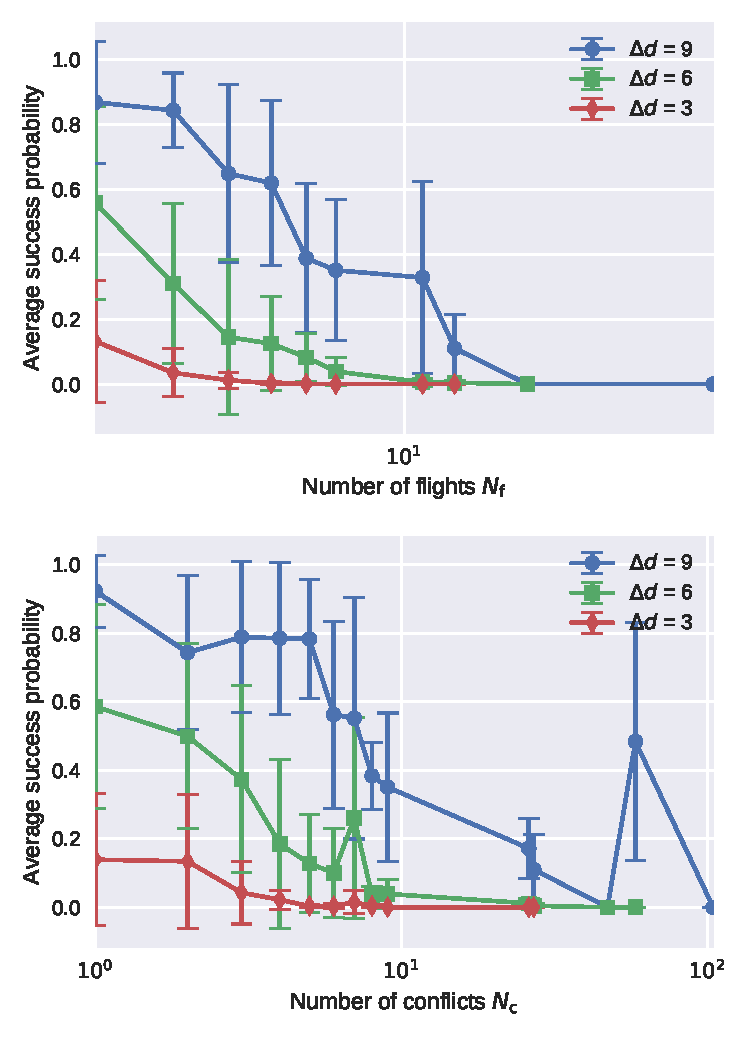
\includegraphics[width=0.45\textwidth]{./pics/annealing_results_success_vs_flights_and_conflicts.pdf}
    \caption{Average success probability for QUBO instances in dependence of the number of flights $N_f$ and the number of conflicts $N_c$. 
             The error bars indicate the standard deviation.
             We used $10000$ annealing runs for each instance and penalty weights $\lambda = \lambda_\text{conflict} = \lambda_\text{unique} \in \{0.5, 1, 2\}$. 
    }
\label{fig:success_probability}
\end{figure}

In figure~\ref{fig:success_probability} the dependence of the average success probability on the number of flights and the number of conflicts is shown.
The average was taken over all successfully embedded QUBO instances with the same number of flights and number of conflicts, respectively.
On can see, that the success probability decreases for larger problem instances as well as for finer discretizations. 
This is a result of the limited precision in the specification of a QUBO on the D-Wave 2X machine~\cite{TODO:D-Wave-precision}.

